\begin{center}
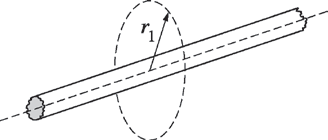
\includegraphics[scale=0.5]{images/img-010-030.png}
\end{center}

% Multiple Choice Question 33
\begin{questions}\setcounter{question}{32}\question
An electric field is produced by the very long, uniformly charged rod shown above. If the strength of the electric field is $E_{1}$ at a distance $r_{1}$ from the axis of the rod, at what distance from the axis is the field strength $\dfrac{E_{1}}{10}$ ?

\begin{oneparchoices}
\choice $\dfrac{r_{1}}{100}$
\choice $\dfrac{r_{1}}{10}$
\choice $\sqrt{10} r_{1}$
\choice $10 r_{1}$
\choice $100 r_{1}$
\end{oneparchoices}\end{questions}

